% This is samplepaper.tex, a sample chapter demonstrating the
% LLNCS macro package for Springer Computer Science proceedings;
% Version 2.20 of 2017/10/04
%
\documentclass[runningheads]{llncs}
%
\usepackage{todonotes}
\newcommand{\remms}[2][]{\todo[color=green!40,#1]{MS:#2}}

\usepackage{graphicx}
\graphicspath{ {./images/} }
% Used for displaying a sample figure. If possible, figure files should
% be included in EPS format.
%
\usepackage{hyperref}
% If you use the hyperref package, please uncomment the following line
% to display URLs in blue roman font according to Springer's eBook style:
\renewcommand\UrlFont{\color{blue}\rmfamily}

\begin{document}
%
%\title{Contribution Title\thanks{Supported by organization x.}}
\title{Natural language generation and processing for the legal domain}
%
%\titlerunning{Abbreviated paper title}
% If the paper title is too long for the running head, you can set
% an abbreviated paper title here
%
\author{Inari Listenmaa\inst{1} \and
Martin Strecker\inst{1} \and
Warrick Macmillan\inst{2}}
%
\authorrunning{I. Listenmaa et al.}
% First names are abbreviated in the running head.
% If there are more than two authors, 'et al.' is used.
%
\institute{Singapore Management University, Centre for Computational Law \\
\email{\{ilistenmaa,mstrecker\}@smu.edu.sg}
%\url{https://cclaw.smu.edu.sg}
\and
University of Gothenburg\\
\email{gusmacwa@student.gu.se}}


%\author{Inari Listenmaa \and Martin Strecker
%\and Warrick Macmillan? % ?
%
% First names are abbreviated in the running head.
% If there are more than two authors, 'et al.' is used.
%
%\institute{Singapore Management University} \\
%\email{\{ilistenmaa,mstrecker\}@smu.edu.sg}}
%
%\authorrunning{I. Listenmaa et al.}}
%
\maketitle              % typeset the header of the contribution
%
%\begin{abstract}
%The abstract should briefly summarize the contents of the paper in 15--250 words.

%\keywords{First keyword  \and Second keyword \and Another keyword.}
%\end{abstract}
%
%
%
The general context of our work is the SMU Centre for Computational Law\footnote{\url{https://cclaw.smu.edu.sg/}} aiming at computerizing legal reasoning in a manner that is both formally precise and intuitively accessible to legal experts. 
The cornerstone is a domain specific language (DSL) for the legal domain, called L4, which can be converted to natural language but is also the basis for formal verification procedures. Inversely, we can also go from natural or close to natural language to a formal DSL. The following highlights essential aspects of this endeavor. 

%to  we seek to generate formally verifiable natural language. 


\textbf{Natural language generation from L4}
Our preliminary efforts, already reported in  \cite{listenmaa-etal-2021-towards,listenmaa2021nlg} 
start from Core L4, with optional (controlled) natural language verbalisations for individual objects and predicates. We have now defined a higher-level variant of the core language, Natural L4 \remms{cannot call that science fiction L4 in a paper...} that, while still being a formal DSL, facilitates human understanding.  Consequently, we describe the \textbf{translation of semi-structured data to natural language}. We also show how Natural L4 can be \textbf{translated to formal logical systems}, in particular combining SAT~/~SMT solvers (\emph{e.g.} Z3\cite{demoura_bjorner_z3_2008}) and Timed Automata (\emph{e.g.} Uppaal \cite{larsen1997uppaal}). 

We compare two approaches, extrapolating ideas from \cite{macmillan2021} to the legal domain. The first tries to generate meaningful natural language from a formal language, desiring \emph{semantic adequacy}. The second approach asks if natural language can be made to fit some well-defined mathematical model, a notion known as \emph{syntactical completeness}.


We explore both the technical differences and their practical implications in the legal domain. If our language fails to be semantically adequate, then the user of the DSL may have an an intensional belief which contradicts the extensional meaning of the some contract, or L4 program. Alternatively, if DSL is syntactically incomplete and the user says something which has no formal meaning, "debugging" the error without explicit knowledge of the DSL will be generally infeasible. Failure to achieve either could not only result in a poor user experience, but have legal consequences for the DSL designers. 
We finally take a glimpse at how we can go still further by translating (controlled) natural language into a Core L4 by translation mechanisms inspired, among others, by \cite{vanEijck2010computationalSemantics,schaefer_kohlhase_glif_2020}.

\todo{TODO: include information that says this is semantically adequate}

%A programming language has formal semantics, and thus the CNL snippets automatically inherit the semantics of their originator. This approach is attractive for producing output that can be fed into formal verification engines. As a trade-off, fluent natural language output requires considerable effort.

\todo{TODO: include explictly that this is the syntactically complete approach}

%\subsubsection{Logical formulas from spreadsheets} In this paper, we compare our initial work to an opposite approach: starting point as a semi-structured natural language input system, using ordinary spreadsheets as the medium. Now the challenge is to derive formal semantics from the initial raw text. 

%
% ---- Bibliography ----
%
% BibTeX users should specify bibliography style 'splncs04'.
% References will then be sorted and formatted in the correct style.
%
% \bibliographystyle{splncs04}
\bibliography{bibliography}
\bibliographystyle{spmpsci}

\newpage
\section*{Brainstorming for later}
Things that won't fit into the 1-page abstract, but are important to discuss/have an idea of. 

\subsection*{Starting from programming language}

\subsubsection*{What Inari/NLG needs}

Described in \cite{listenmaa-etal-2021-towards}. %,listenmaa2021nlg}. 
We have done it for tiny examples, scaling up needs a lot of work and probably some kind of ontology/real world knowledge base. Importantly, we can't (with the methods tried so far) do NLG from purely programming language input: all we've accomplished depends on additional NL fragments to annotate the programming language concepts.

\subsubsection{What Martin/FV needs}

Nothing? It's already a programming language with formal semantics.


\subsection*{Starting from spreadsheets/semi-structured NL} 

\subsubsection{What it is exactly} It is a mixture of fixed keywords and free text, see picture\footnote{The exact syntax is changing all the time, so don't take the examples too seriously.}. 

\noindent 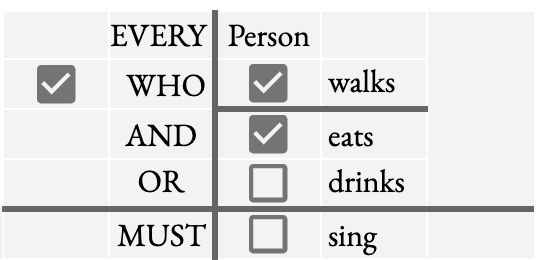
\includegraphics[width=80mm]{spreadsheets.png}


The free text snippets have varying levels of structure and complexity, see another example below. You can put linebreaks and separate the text in to ad hoc \texttt{key}:\textit{value} pairs, like \texttt{with}:\textit{a message}. \\

\noindent 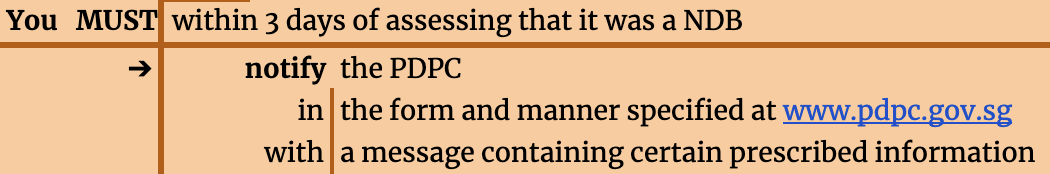
\includegraphics[width=123mm]{images/spreadsheets-complex.png}

\noindent The bit about "notify the PDPC in the form … with a message …" is already structured, so we can extract---even without any NLP tool---that \textit{notify} is the main predicate, and \textit{the PDPC} is probably the most important argument, because it's on the same line with \textbf{notify}. 

This happens to line up naturally with a traditional constituency-based description of the English verb phrase: ``the PDPC'' is a direct object, i.e. an obligatory argument to \textbf{notify}, whereas ``\textbf{in} the form \dots'' and ``\textbf{with} a message \dots'' are optional modifiers, more specifically adverbials. But in the general case, the key and the value  can be any strings. In fact, \textbf{in} and \textbf{with} are not reserved words---only the words in all caps are.

The spreadsheet is parsed into a Haskell datatype, which retains the separation of keys (``with'') and values (``a message \dots''). Here's an example of a rule that says \textit{every singer must pay the king \$20}.

\begin{verbatim}
    { every = "Singer"
    , deontic = DMust
    , action = ( "pay" :| [] ) :|
                   [ "to"     :| [ "the King" ]
                   , "amount" :| [ "$20" ]
                   ]
    }
\end{verbatim}

Here's another example which says that every person may eat a potato, if the potato is tasty and not green: 

\begin{verbatim}
    { every = "person"
    , cond = All
               [ ( "tasty(potato)" :| [] ) :| [] )
               , Not ( "green(potato)" :| [] ) :| [] )
               ]
    , deontic = DMay
    , action = ( "eat potato" :| [] ) :| []
    }
\end{verbatim}

There is some non-natural syntax: \texttt{tasty(potato)} is coming from the spreadsheet and reproduced verbatim. (I assume that ``a/the potato is tasty'' can be easily desugared into \texttt{tasty(potato}.) As of now, all of these things are just strings, and there is no connection between the potato in \texttt{eat potato} and \texttt{tasty(potato)}. If this is supposed to be natural language, it seems rather risky to generally assume that all strings of the same form refer to the same entity.

\subsubsection{What Inari/NLG needs}

For NLG purposes, I'm so far pretty happy with the format. I don't really care that the key/value pairs are linguistically inconsistent: I can always get the linguistically meaningful parse by flattening it to a string and then parsing it with a real NLP framework. For me, a relevant problem is to know when to keep the key and when to omit. For example:

\begin{itemize}
    \item \textit{pay the king \$20} is more natural than \textit{pay the king amount \$20}, but both are grammatical
    \item \textit{notify the PDPC with a message} is the only grammatical option; \textit{notify the PDPC a message} is nonsense
\end{itemize}

It would be kind of nice to know if all instances of ``potato'' refer to the same potato, for the sake of deciding whether to call things  ``a potato'' or ``the potato''. But this is not as crucial as other things.

\subsubsection{What Martin/FV needs}


Outline of the structure of a full paper:
\begin{enumerate}
    \item Natural language production from L4
    \item Translation of semi-structured data coming from spreadsheets to NL
    \item Translation to logic / automata 
    \item Free Natural language input to logical form
\end{enumerate}



Some kind of logical form from the ad hoc structure. Martin has been looking into Montague semantics and thinks it looks nice. Inari has no idea how that stuff works.

Martin's answer to ``what do you need'' (re: \textit{pay the king \$20} example):
\begin{quote}
{
\it
I would not have a unique response. There is not one way to translate a sentence - it depends on how one wants to model a scenario: In some cases, "pay" could be a two- or three-place predicate (who / to whom / amount), in some cases, it might be a transition in an automaton. And this is something the NLG processor cannot know - this has to be fixed in advance by the human modeller, in some kind of ontology / terminology / mapping.
}
    \end{quote}

Some things we have briefly looked at. NLG team plans to first parse the free text with UD parser, and then convert them to GF, so both UD- and GF-based logic/semantic layer is possible. Although, the planned GF grammar is just going to be a loose transformation of the UD structure.

\begin{itemize}
    \item UDepLambda \url{https://github.com/sivareddyg/UDepLambda}, but Martin was initially not impressed by how the logical forms look. Is there a way to convert them into something that looks more like Montague grammar?
    \item GLIF \url{https://github.com/KWARC/GLIF}. Based on Frederik's talk in GFSS2021, the MMT-based logic layer is bootstrapped from the GF grammar. This works nicely for grammars that look like this:
    
    \begin{verbatim}
     abstract Grammar = {
      cat
        Person ; Action ; Sentence ;

      fun
        john, mary : Person ;
        run, be_happy : Action ;
        make_sentence : Person -> Action -> Sentence ;
        and : Sentence -> Sentence -> Sentence ; }
    \end{verbatim}
    
    This translates into logic formulas that look like \texttt{run(john)}, \texttt{be\_happy(mary)}. But the grammar used for parsing the free text snippets will not look like that---either it's a variant of the GF RGL, or a UD-based layer on top of it. The functions look like this:
    
    \begin{verbatim}
    --"once an organisation is aware of a data breach ;
    root_advmod_nsubj_cop_obl : root -> advmod -> nsubj -> cop -> obl -> UDS ;
    \end{verbatim}
    
    If this syntax doesn't work for our purposes, we'll probably just use raw RGL abstract syntax for the parsing. Another option would be to add yet another application layer, which mimics the Haskell data types of the parsed spreadsheet---the one with fields like \texttt{every, cond, deontic, action} etc.
    
    \item FrameNet to list the potential arguments of a predicate?
\end{itemize}

\subsubsection{How could Warrick help}

\begin{itemize}
    \item General knowledge about logical semantics and natural language understanding, relevant prior work to learn from
    \item Thoughts about syntactic completeness and semantic adequacy, and how they apply to the research problems stated in this document
    \item \dots
\end{itemize}

\end{document}
